\documentclass{article}
\usepackage{tikz}
\begin{document}

\section{LaTeX Editor with TikZ Support}

This editor supports various LaTeX elements:

\begin{enumerate}
  \item Math formulas: $E = mc^2$
  \item Tables and figures
  \item TikZ diagrams
  \item Lists and sections
\end{enumerate}

\subsection{Math Example}

Display math:
$$\int_{0}^{1} x^2 dx = \frac{1}{3}$$

\begin{align}
a &= b + c \\
  &= d + e
\end{align}

\subsection{Table Example}

\begin{table}[h]
  \begin{center}
  \begin{tabular}{|c|c|c|}
      \hline
      \textbf{x} & \textbf{f(x)} & \textbf{Notes} \\
      \hline
      0 & 1 & Base case \\
      1 & 1 & Base case \\
      2 & 2 & $f(1) + f(0)$ \\
      3 & 3 & $f(2) + f(1)$ \\
      4 & 5 & $f(3) + f(2)$ \\
      \hline
  \end{tabular}
  \caption{Fibonacci Sequence}
  \end{center}
\end{table}

\subsection{TikZ Example}

Basic circle:

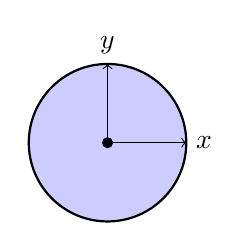
\begin{tikzpicture}
\draw[thick, fill=blue!20] (0,0) circle (1cm);
\draw[->] (0,0) -- (1,0) node[right] {$x$};
\draw[->] (0,0) -- (0,1) node[above] {$y$};
\fill (0,0) circle (2pt);
\end{tikzpicture}

Function plot:

\begin{tikzpicture}
\draw[->] (-0.5,0) -- (4,0) node[right] {$x$};
\draw[->] (0,-0.5) -- (0,4) node[above] {$y$};
\draw[domain=0:3, smooth, variable=\x, blue, thick] plot ({\x}, {\x*\x});
\node at (2,3) {$y = x^2$};
\end{tikzpicture}

\end{document}